% WACV 2027 version of the MMCTL manuscript.
% Ported from the IEEEtran draft bare_jrnl_new_sample4.tex.
% Revision changes vs paper_files/bare_jrnl_original_baseline.tex are wrapped in
% \new{...} / {\color{red} ...} and render in red.
\documentclass[10pt,twocolumn,letterpaper]{article}

\usepackage[review,algorithms]{wacv}   % REVIEW version, algorithms track

%
% --- inline annotations
%
\newcommand{\red}[1]{{\color{red}#1}}
\newcommand{\todo}[1]{{\color{red}#1}}
\newcommand{\TODO}[1]{\textbf{\color{red}[TODO: #1]}}
% --- disable by uncommenting  
% \renewcommand{\TODO}[1]{}
% \renewcommand{\todo}[1]{#1}


   % defines \red, \todo, \TODO

% Packages used by the ported body
\usepackage{amsmath,amsfonts,amssymb}
\usepackage{array}
\usepackage{booktabs}
\usepackage{multirow}
\usepackage{graphicx}
\usepackage{xcolor}
\graphicspath{{../}{./}}   % so figures/<name> resolves to ../figures/<name>

% Red highlighting macro for newly added revision content (matches the IEEEtran draft)
\newcommand{\new}[1]{\textcolor{red}{#1}}

\definecolor{wacvblue}{rgb}{0.21,0.49,0.74}
\usepackage[pagebackref,breaklinks,colorlinks,allcolors=wacvblue]{hyperref}

\def\wacvPaperID{*****}
\def\confName{WACV}
\def\confYear{2027}

\title{Learning Annotation-Driven Latent Structure for Multi-Modal Fusion}

\author{Meilun Zhou \quad Aditya Dutt \quad Alina Zare\\
University of Florida, Gainesville, FL, USA\\
{\tt\small \{meilun.zhou, aditya.dutt\}@ufl.edu \quad azare@ufl.edu}}

\begin{document}
\maketitle

\begin{abstract}
Learning shared representations from heterogeneous sensing modalities requires explicitly aligning information that differs in scale, structure, and semantics. Most multi-modal fusion methods rely on downstream task optimization to create cross-modal structure. This work introduces Multi-Modal Continuous Triplet Loss (MMCTL), a representation learning framework that constructs a shared latent space by enforcing similarity relationships derived directly from task annotations. Each modality is processed by a dedicated encoder that maps modality-specific inputs into a common embedding space. MMCTL then applies a continuous triplet loss that compares pairs of samples using annotation-defined similarity, where similarity scores are computed from a weighted combination of classification labels and continuous attributes such as bounding box geometry and object height. Experiments on the AWIR and NEON remote sensing datasets show that this multi-modal alignment yields more coherent and consistently structured latent geometry than unimodal or task-driven fusion approaches.
\end{abstract}

\section{Introduction}
Multi-modal remote sensing relies on fused representations to integrate complementary sensing modalities \cite{chen2024novel}. Most fusion approaches are developed under a task-driven objective, where fusion is optimized to minimize downstream prediction losses such as classification or regression \cite{bai2025task}. This paradigm can yield strong task accuracy, but it shapes the embedding space only indirectly: distances among samples are not constrained to reflect annotation-defined similarity, so latent geometry becomes a byproduct of whichever prediction objectives are minimized rather than an explicit model of how annotated objects relate.

This gap is especially consequential when supervision mixes categorical labels with continuous attributes. Remote sensing annotations frequently encode size, height, or spatial extent alongside semantic class \cite{sun2023single}. Binary contrastive and classical triplet formulations treat pairs as simply similar or dissimilar \cite{khosla2020supervised}, which discards graded relationships among continuously annotated samples and can flatten intra-class geometric variation. Task-driven fusion likewise encourages decision boundaries that are sufficient for prediction, but does not require that embedding distances remain ordered by continuous annotation proximity across modalities. As a result, fused representations may score well on trained heads while failing to expose an interpretable, annotation-aligned geometry for retrieval, transfer, or multi-attribute reasoning \cite{saidi2024deep}.

This work introduces Multi-Modal Continuous Triplet Loss (MMCTL), which treats multi-modal representation learning as constructing a shared latent space whose geometry is driven by a joint annotation vector. Building on shared-manifold multi-sensor triplets \cite{dutt2022shared} and continuous multi-annotation metric learning \cite{zhou2025multi,kim2019deep}, MMCTL organizes heterogeneous modality embeddings so that relative distances track continuous annotation similarity rather than binary match status or task-loss residuals. Critically, MMCTL uses the \emph{same} annotation sources available to task-driven baselines; the distinction is inductive bias---geometry matching in a shared multi-modal space versus optimizing prediction losses alone. As shown in Fig.~\ref{fig:emb_awir}, paired RGB and thermal embeddings of the same objects occupy nearby regions while class identity and continuous geometric attributes remain structured, in contrast to fusion methods where cross-modal alignment emerges only indirectly from downstream objectives.

% \section{Introduction}
% Multi-modal remote sensing typically relies on shared embeddings to integrate different sensing modalities. Most existing fusion approaches focus on improving downstream task performance through architectural coupling or task-specific supervision \cite{houdre2025promm}. While these strategies achieve high task accuracy, they do not explicitly control the geometric structure of the learned embedding space. As a result, representations may collapse nuanced semantic relationships when supervision is heterogeneous or continuous \cite{liu2020global}. Additionally, supervised models are often task-specific, which may limit their generalization across different geographic or temporal domains \cite{houdre2025promm}.

% Most embedding-level fusion methods rely on contrastive formulations that treat all mismatched samples as equally dissimilar. This binary assumption that classifies pairs as either "similar" or "dissimilar" is poorly suited for remote sensing annotations that include continuous attributes such as elevation, moisture content, or biophysical variables. In contrastive frameworks, the reliance on binary pairs can be problematic in remote sensing because diverse images may belong to the same semantic class and lead to encoder collapse or non-informative constant embeddings \cite{choudhury2025rejepa}. This often results in a collapsed embedding space where intra-class variations are ignored, and inter-class distances fail to reflect physical reality \cite{liu2020global}. Furthermore, as supervision sources increase, conflicting task gradients or negative transfer, can distort the shared embedding geometry by forcing shared parameters to optimize for opposing directions \cite{xie2023co, liu2021conflict}. 

% We propose a Continuous Triplet Loss to preserve annotation-grounded geometry rather than enforcing binary similarity. By aligning relative distances in the embedding space with continuous similarity measured in annotation space, this formulation has been shown to learn effective representations under continuous supervision \cite{kim2019deep}. This work applies Continuous Triplet Loss in a multi-modal setting to jointly coordinate embeddings from multiple sensing modalities in a shared latent space using annotation-driven geometry rather than task objectives. As illustrated in Fig.~\ref{fig:emb_awir}, MMCTL coordinates RGB and thermal embeddings from the AWIR dataset so that samples corresponding to the same object are aligned across modalities while preserving semantic separation by class and smooth variation with box size. In contrast, simple concatenation produces disjoint modality clusters with limited cross-modal alignment, and DeepSet fusion \cite{reiter2020deep} fails to clearly separate classes or reflect geometric attributes such as box size. 

\begin{figure*}[!htb]
    \centering
    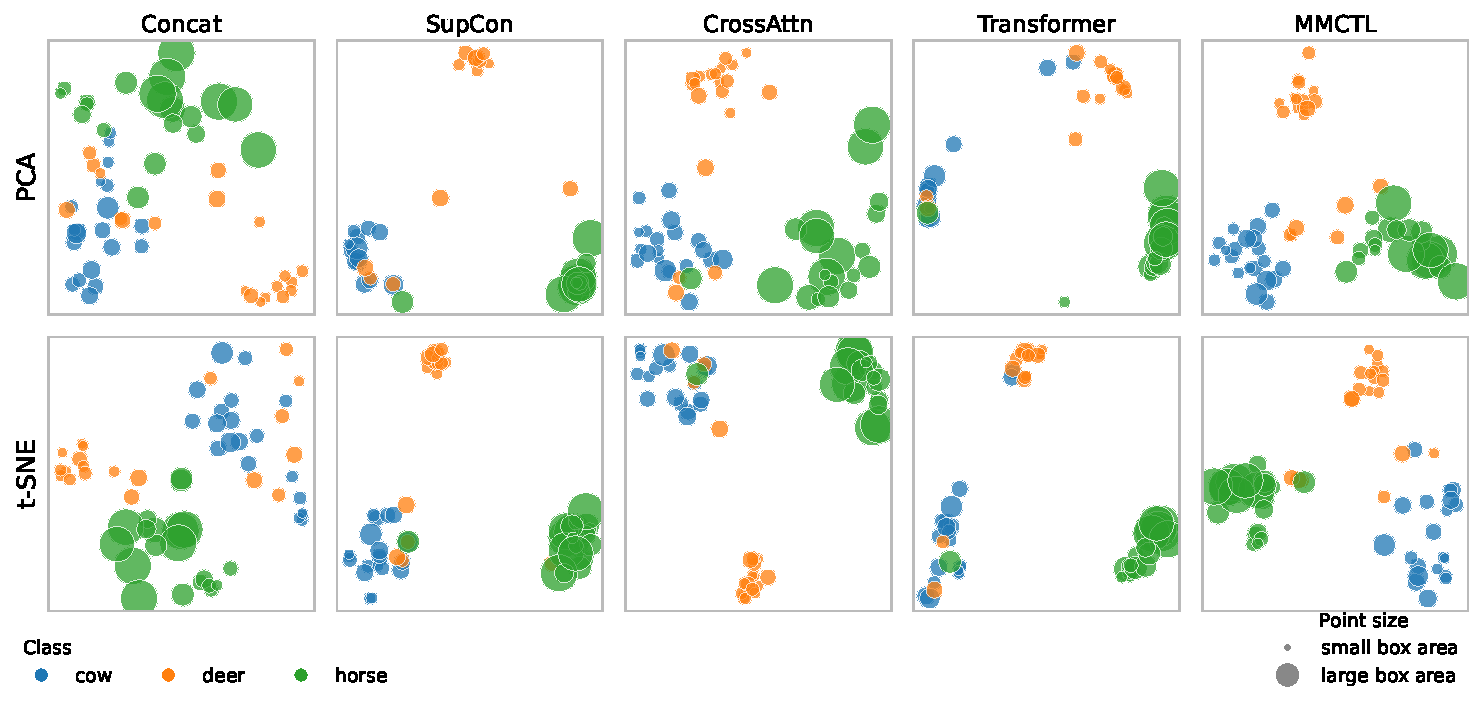
\includegraphics[width=\textwidth]{figures/awir_embedding_space.pdf}
    \caption{\new{AWIR embedding space across fusion methods (Concat, SupCon, cross-attention, Transformer, MMCTL), projected with PCA (top) and t-SNE (bottom). Points are colored by class label (cow, deer, horse) and sized by bounding-box area. Task-driven fusion baselines mix classes or show no ordered size gradient, whereas MMCTL yields class-separated clusters in which point size varies smoothly within and across clusters, reflecting the annotation-aligned continuous geometry.}}
    \label{fig:emb_awir}
\end{figure*}

\section{Related Work}
\label{sec:related}

\red{Binary supervised contrastive and cross-modal triplets define positives by class or view co-membership with a fixed margin \cite{khosla2020supervised,dutt2022shared}. Continuous metric learning instead couples distances to graded targets \cite{kim2019deep}, including adaptive-margin triplets \cite{ha2021adaptive}. Shared-manifold multi-sensor triplets align heterogeneous modalities for fusion with missing data \cite{dutt2022shared}; our prior multi-annotation continuous triplet organizes a \emph{unimodal} detector from joint class and box labels \cite{zhou2025multi}.}

\red{MMCTL contributes: (i)~a joint annotation vector with normalization and task weights (Eqs.~\eqref{eq:ann-norm}--\eqref{eq:ann-concat}); (ii)~a margin-free continuous triplet with adaptive gap $D(\mathbf{y}_a,\mathbf{y}_q)-D(\mathbf{y}_a,\mathbf{y}_p)$ (Eq.~\eqref{eq:mm-adaptive}); (iii)~pairwise distance alignment (Eq.~\eqref{eq:mm-reg}); (iv)~a multi-modal shared space where same-object, different-modality pairs have zero annotation distance. Relative to \cite{zhou2025multi}, MMCTL targets fusion geometry; relative to SupCon or fixed-margin triplets, it replaces hard partitions with annotation-ordered continuous constraints.}

\section{Methodology}
\label{sec:methodology}

\subsection{Problem Setup}
\label{subsec:problem-setup}

Consider a multi-modal dataset with $M$ sensing modalities and $N$ instances.
Let $\mathbf{x}_n^{(m)} \in \mathbb{R}^{d_m}$ denote the input for instance
$n \in \{1,\dots,N\}$ from modality $m \in \{1,\dots,M\}$, where $d_m$
denotes the modality-specific input dimensionality.

Each instance is associated with $T$ annotation sources.
For task $t \in \{1,\dots,T\}$, the annotation for instance $n$ is represented
by a row vector
\[
\mathbf{y}^{t}_{n}
=
\big[
y^{t}_{n,1}\;\; y^{t}_{n,2}\;\; \dots\;\; y^{t}_{n,L_t}
\big]
\in \mathbb{R}^{1 \times L_t},
\]
where $L_t$ denotes the number of annotation features for task $t$.

To ensure comparability across annotation sources with different scales,
each annotation feature is normalized independently to the interval $[0,1]$
using statistics computed from the training set only.
Let $\mathcal{N}_{\mathrm{train}} \subset \{1,\dots,N\}$ denote the index set of
training instances.

For each task $t$ and annotation feature index $\ell \in \{1,\dots,L_t\}$, define the
training-set extrema
\[
\mu^{t}_{\min,\ell}
=
\min_{n \in \mathcal{N}_{\mathrm{train}}} y^{t}_{n,\ell},
\qquad
\mu^{t}_{\max,\ell}
=
\max_{n \in \mathcal{N}_{\mathrm{train}}} y^{t}_{n,\ell}.
\]

\noindent Normalization is applied feature-wise as
\begin{equation}
\label{eq:ann-norm}
\tilde{y}^{t}_{n,\ell}
=
\frac{
y^{t}_{n,\ell}
-
\mu^{t}_{\min,\ell}
}{
\mu^{t}_{\max,\ell}
-
\mu^{t}_{\min,\ell}
},
\qquad
\forall \ell \in \{1,\dots,L_t\}.
\end{equation}

\noindent The same normalization parameters are reused unchanged for validation and test instances. After normalization, annotation vectors are rescaled to account for differences in dimensionality across tasks.
Let
\[
L_{\max} = \max_{t \in \{1,\dots,T\}} L_t .
\]
Each normalized annotation vector is scaled and weighted as
\begin{equation}
\label{eq:ann-weight}
\hat{\mathbf{y}}^{t}_{n}
=
w_t \, \tilde{\mathbf{y}}^{t}_{n}\, \frac{L_{\max}}{L_t},
\end{equation}
where $w_t \ge 0$ is a fixed hyperparameter controlling the influence of task $t$. Feature-wise min--max normalization and the $L_{\max}/L_t$ length correction are therefore already encoded in Eqs.~\eqref{eq:ann-norm}--\eqref{eq:ann-weight}; the only free annotation knobs are the task weights $\{w_t\}$. \red{In the main experiments we fix $w_{\text{class}}{=}0.5$ on AWIR and $w_{\text{class}}{=}1.0$ on NEON (with continuous-task weights at $1.0$) to balance semantic and geometric sources.}

The final joint annotation vector for instance $n$ is constructed by horizontal
concatenation:
\begin{equation}
\label{eq:ann-concat}
\mathbf{y}_{n}
=
\big[
\hat{\mathbf{y}}^{1}_{n}
\;\;
\hat{\mathbf{y}}^{2}_{n}
\;\;
\dots
\;\;
\hat{\mathbf{y}}^{T}_{n}
\big]
\in
\mathbb{R}^{1 \times L},
\end{equation}
where $L = \sum_{t=1}^{T} L_t$.
This joint annotation vector defines a unified similarity space whose geometry
reflects relationships across all annotation sources.


\subsection{Shared Latent Space with Modality-Specific Encoders}
\label{subsec:shared-latent-space}
Multi-modal observations provide complementary and non-redundant information about each instance, as different sensing modalities capture distinct physical, spectral, or geometric properties. Leveraging these complementary cues requires a representation that preserves modality-specific information while enabling direct comparison and alignment across modalities. To this end, each modality is processed by a dedicated encoder that maps modality-specific inputs into a shared latent space.

Each modality is processed by a dedicated encoder
$e_m(\cdot)$ that maps modality-specific inputs into a shared latent space.
For instance $n$ and modality $m$,
\begin{equation}
\mathbf{z}_n^{m}
=
e_m\!\left(\mathbf{x}_n^{m}\right),
\qquad
\mathbf{z}_n^{m} \in \mathbb{R}^{F},
\end{equation}
where $F$ denotes the shared embedding dimension.

Similarity in both annotation space and latent space is measured using cosine
distance,
\begin{equation}
D(\mathbf{u},\mathbf{v})
=
1 -
\frac{
\mathbf{u}^{\top}\mathbf{v}
}{
\|\mathbf{u}\|_2 \|\mathbf{v}\|_2
}.
\end{equation}

Triplets are formed with a \emph{batch-all} strategy. Within each mini-batch, every index may serve as an anchor $a$. For that anchor, a pair $(p,q)$ is a valid (positive, negative) pair if and only if
\begin{equation}
\label{eq:triplet-order}
D(\mathbf{y}_a,\mathbf{y}_p)
<
D(\mathbf{y}_a,\mathbf{y}_q).
\end{equation}
Positives and negatives are therefore defined solely by annotation-distance ordering: any sample closer to the anchor in joint annotation space than another is treated as relatively more similar. There is \emph{no} hard similarity threshold that partitions pairs into absolute positives and negatives, and no class-equality rule beyond what is already encoded in $\mathbf{y}_n$.

Let $K$ denote the number of valid triplets in a batch under this batch-all construction. The multi-modal continuous triplet loss is
\begin{equation}
\label{eq:mm-adaptive}
\begin{aligned}
\mathcal{L}_{\text{mm\_adaptive}}
=
\sum_{k=1}^{K}
\Big(
& \max\!\big(
D(\mathbf{z}_{a_k},\mathbf{z}_{p_k})^2
-
D(\mathbf{z}_{a_k},\mathbf{z}_{q_k})^2 \\
& \quad +
D(\mathbf{y}_{a_k},\mathbf{y}_{q_k})
-
D(\mathbf{y}_{a_k},\mathbf{y}_{p_k}),
\, 0
\big)
\Big).
\end{aligned}
\end{equation}
There is no fixed margin hyperparameter. The term $D(\mathbf{y}_{a},\mathbf{y}_{q})-D(\mathbf{y}_{a},\mathbf{y}_{p})$ acts as an adaptive, annotation-derived margin: the required embedding separation equals the annotation-distance gap for that triplet.

To encourage consistency between annotation-defined geometry and embedding
geometry, a regularization term enforces pairwise distance alignment,
\begin{equation}
\label{eq:mm-reg}
\begin{aligned}
\mathcal{L}_{\text{mm\_reg}}
=
\sum_{k=1}^{K}
\Big(
& \left(
D(\mathbf{z}_{a_k},\mathbf{z}_{p_k})
-
D(\mathbf{y}_{a_k},\mathbf{y}_{p_k})
\right)^2 \\
& \quad +
\left(
D(\mathbf{z}_{a_k},\mathbf{z}_{q_k})
-
D(\mathbf{y}_{a_k},\mathbf{y}_{q_k})
\right)^2
\Big).
\end{aligned}
\end{equation}
The final Multi-Modal Continuous Triplet Loss is
\begin{equation}
\mathcal{L}_{\text{mm\_ctl}}
=
\mathcal{L}_{\text{mm\_adaptive}}
+
\mathcal{L}_{\text{mm\_reg}}.
\end{equation}

When the same instance is observed across multiple modalities, identical joint
annotation vectors yield zero annotation distance. This property encourages
embeddings of the same physical object from different sensing modalities to
align in the shared latent space while preserving continuous variation across
distinct instances.


\subsection{Modality-Specific Encoder Architecture}

Each sensing modality is first encoded using a dedicated convolutional autoencoder trained independently with a standard reconstruction objective. This design allows each encoder to specialize in extracting features aligned with the physical characteristics and information content of its corresponding modality, without imposing cross-modal constraints during representation learning.

For hyperspectral imagery, the encoder architecture emphasizes spectral feature extraction. The network uses $1 \times 1$ convolutions to model per-pixel spectral relationships, followed by densely connected layers that capture higher-order spectral interactions. Global average pooling is applied at the final convolutional stage to aggregate spectral responses into a fixed-length representation. For RGB, thermal, and LiDAR modalities, the encoder architecture emphasizes spatial structure. These encoders use spatial convolutions organized into dense blocks to capture local and contextual spatial patterns present in each modality. Global average pooling is applied after the final dense block to produce a compact representation that is invariant to spatial resolution.

In all cases, the encoder outputs a $1024$-dimensional latent embedding vector. Modality-specific autoencoders are first pretrained independently with reconstruction objectives. For all fusion methods evaluated here---including concatenation, \red{SupCon, cross-attention, Transformer fusion,} and MMCTL---those modality encoders are then frozen, and fusion operates on fixed embeddings. This two-stage freeze is a \emph{fair fusion evaluation protocol}: it isolates shared-space organization from differences in modality-specific feature learning, so that downstream gaps reflect fusion geometry rather than unequal encoder capacity. Under this protocol, MMCTL trains only the shared multi-modal organization with annotation-derived distance supervision (Section~\ref{subsec:shared-latent-space}); after MMCTL training, the resulting embeddings are frozen and lightweight task heads are trained separately, as shown in Fig.~\ref{fig:MMCTL_Training_Architecture}. \red{A controlled end-to-end comparison on NEON (Section~\ref{subsec:weight-e2e}) confirms that unfreezing the modality encoders does not improve classification over this frozen protocol, so freezing is used throughout the main tables.}

\begin{figure}[!htb]
    \centering
    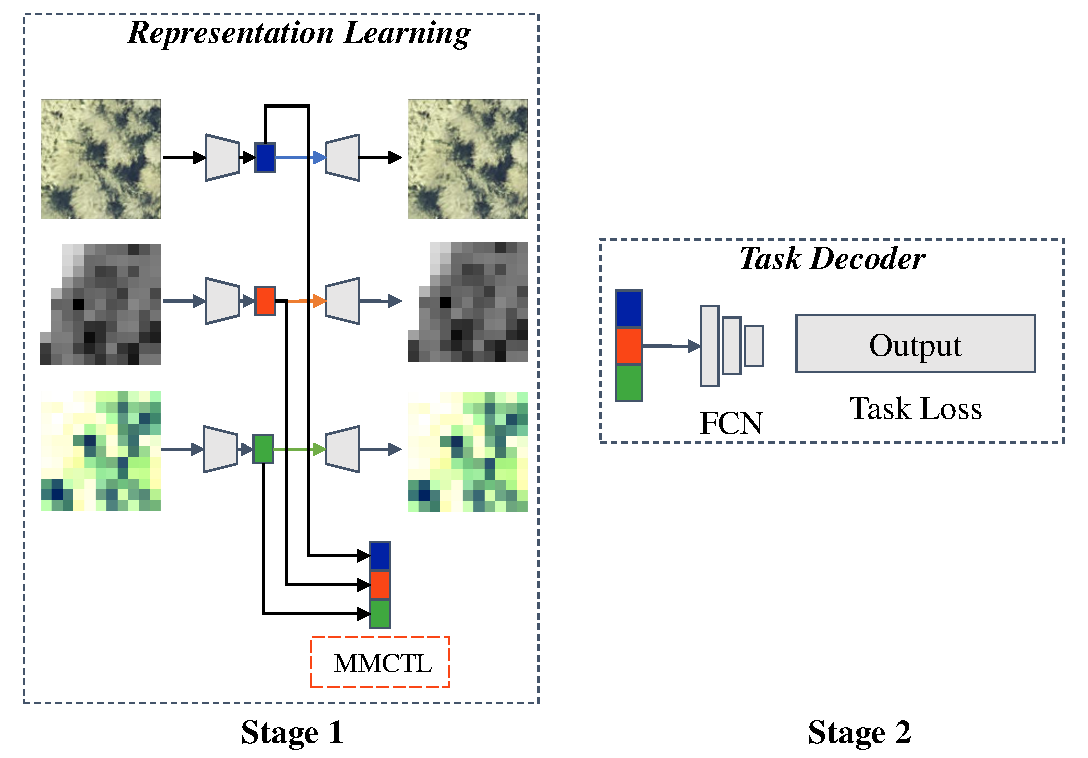
\includegraphics[width=\columnwidth]{figures/MMCTL-Framework-Figure.pdf}
    \caption{Two-stage MMCTL training on NEON under the frozen-encoder fusion protocol. Modality-specific encoders are pretrained and frozen; MMCTL organizes the shared latent space with Continuous Triplet Loss over a joint annotation vector; task-specific heads are then trained independently to assess representation quality.}
    \label{fig:MMCTL_Training_Architecture}
\end{figure}

\section{Experiments}

\subsection{Datasets and Modalities}
\label{subsec:datasets}

Experiments are conducted on two remote sensing datasets that differ in sensing modalities, spatial resolution, and annotation structure. These datasets provide complementary test cases for evaluating multi-modal embedding fusion under heterogeneous sensing conditions.

The first dataset is Animal Wildlife Image Repository (AWIR) \cite{samiappan2024aerial, zhou2025multi}, which contains paired RGB and thermal imagery observing the same objects and spatial regions. RGB provides high-resolution visual appearance, while thermal supplies complementary temperature-based cues. The data processing follows the existing pipeline \cite{zhou2025multi}. The NEON dataset is derived from the NeonTreeEvaluation Benchmark \cite{Weinstein_Marconi_White_2022} and includes aligned RGB, hyperspectral, and LiDAR data from NEON airborne products. Tree crowns are centered on stem locations with species labels from NEON vegetation structure data \cite{NEON_vegetation_structure}. Species labels are provided per stem, crown polygons yield geometric attributes, and height statistics are computed from LiDAR-derived canopy height models, including minimum, maximum, mean, and standard deviation of height. We extract $6\times6$ patches at $1\,\mathrm{m}$ for hyperspectral and CHM and $60\times60$ patches at $10\,\mathrm{cm}$ for RGB, then apply Min-Max normalization using training statistics.

\subsection{Experimental Setup}
Evaluation targets embedding-level fusion under a two-stage frozen-encoder protocol (Section~\ref{sec:methodology}). For all comparison methods, modality-specific encoders are frozen and fusion operates on fixed embeddings. Task-driven fusion methods observe the same annotation sources as MMCTL, but consume them through supervised prediction losses during fusion training; MMCTL instead uses those annotations to define continuous distances for geometry matching (Section~\ref{subsec:shared-latent-space}). The claim is therefore not that MMCTL forgoes labels, but that it applies a different inductive bias to the same label sources. Datasets are split into $50\%$ training and $50\%$ test sets, with the test set excluded from model selection. Within the training split, $k$-fold cross-validation is used for model selection and uncertainty reporting: $8$ folds for AWIR and $5$ folds for NEON. All splits use a fixed random seed, and each reported mean~$\pm$~std is computed across these folds (i.e., the ``runs'' in figure captions are the CV folds). Categorical annotations use a fixed weight of $w_{\text{class}} = 0.5$ in the joint annotation vector for the AWIR dataset and $1.0$ for the NEON dataset to balance with continuous annotations.

\red{Comparisons include concatenation and three stronger fusion baselines requested for this revision: supervised contrastive fusion (SupCon) \cite{khosla2020supervised}, cross-attention pooling, and a small Transformer encoder over modality tokens. Concatenation stacks modality embeddings and remains untrained. SupCon learns a projection of the concatenated embeddings with class-supervised contrastive loss. Cross-attention and Transformer fusion are trained with classification and continuous regression task supervision. These methods contrast with MMCTL, which organizes latent geometry using annotation-derived similarity rather than prediction losses alone.}

Next, task heads are optimized using supervised losses appropriate to each task, with identical architectures and optimization settings across all fusion methods. Training runs for up to $3000$ epochs with early stopping based on validation performance and a patience of $1000$ epochs. Optimization uses Adam with a learning rate of $10^{-3}$ and weight decay of $10^{-4}$. Batch size is set to $4$ for AWIR with no gradient clipping applied, while NEON uses a batch size of $32$ with gradient clipping enabled at a norm of $5$. Task heads use a shallow multilayer perceptron for both classification and regression tasks. Code for reproducing all experiments can be found at
\href{https://github.com/GatorSense/MMCTL}{github.com/GatorSense/MMCTL}.

\new{\noindent\textbf{Reproducibility.} AWIR and NEON tables use released full-set embeddings ($N{=}240$ AWIR; $N{=}592$ NEON) with independently trained unimodal encoders and MMCTL. SupCon, cross-attention, and Transformer fusion are trained on frozen unimodal embeddings under a $50/50$ holdout plus $k$-fold protocol ($8$ AWIR / $5$ NEON) and paper task-head settings (Adam, $3000$ epochs, patience $1000$).}

\subsection{Latent Space Quality Metrics}
\label{sec:latent_space_quality_metrics}
{\color{red}
Latent space quality is evaluated with two standard, directly interpretable metrics: one that gauges categorical class separation and one that gauges how faithfully the geometry represents differences in the continuous annotations. Both are computed on L$_2$-normalized embeddings with cosine geometry, matching the MMCTL training distance.

\noindent\textbf{Class separation.}
We report the silhouette coefficient over class labels. For sample $i$ with class $c_i$, let $a_i$ be its mean cosine distance to other same-class embeddings and $b_i$ its mean cosine distance to the nearest other class; the silhouette is
\begin{equation}
\label{eq:silhouette}
\mathrm{Sil}
=
\mathbb{E}_i\!\left[
\frac{b_i - a_i}{\max(a_i, b_i)}
\right]
\in [-1, 1],
\end{equation}
where higher values indicate more compact, better-separated classes.

\noindent\textbf{Continuous-annotation representation.}
To measure whether embedding geometry reflects graded annotation differences, we correlate pairwise distances. For supervision source $s \in \{\mathrm{box}, \mathrm{pos}, \mathrm{height}\}$, let $d_E(i,j)$ be the cosine distance between embeddings and $d_s(i,j)$ the Euclidean distance between the corresponding annotation vectors. The distance-preservation score is the Spearman rank correlation
\begin{equation}
\label{eq:spearman}
\rho_s
=
\operatorname{Spearman}\big(
\{ d_E(i,j) \}_{(i,j)},\
\{ d_s(i,j) \}_{(i,j)}
\big)
\in [-1, 1],
\end{equation}
over all evaluation pairs, where higher values indicate that samples close in annotation space are embedded close together. Metrics are computed on each held-out cross-validation fold and reported as mean~$\pm$~std.
}



\subsection{Experimental Results}
\new{\noindent\textbf{Latent-space quality.} Latent space quality is first evaluated using the silhouette and distance-preservation metrics defined in Subsection~\ref{sec:latent_space_quality_metrics}. Table~\ref{tab:latent_alignment} compares class separation and continuous-annotation representation across unimodal encoders, fusion methods, and MMCTL.}

\new{No single baseline is coherent on both fronts. Class-supervised fusion (SupCon, Transformer) attains the highest class silhouette but collapses continuous geometry, with position/height correlations near zero or negative (e.g., AWIR position $\rho\!=\!-0.02$ for both). Conversely, the modality that directly senses an attribute can lead its continuous column---LiDAR attains the best NEON height correlation ($\rho\!=\!0.571$)---yet separates classes poorly (silhouette $-0.23$). MMCTL is the only method that is simultaneously strong on both: it gives the best continuous representation on AWIR (box $\rho\!=\!0.278$, position $\rho\!=\!0.223$, the latter far above every baseline), the second-best class silhouette on NEON behind SupCon, and the second-best NEON height correlation behind LiDAR. Rather than maximizing any one column, annotation-driven multi-modal supervision yields a balanced, coherent geometry that reflects both semantic classes and continuous attributes at once.}


\newcommand{\err}[1]{\,\scriptstyle\pm\,\!#1}

\begin{table}[t]
\centering
\caption{\new{
Embedding-space quality across datasets. \textbf{Sil} is the class-label silhouette coefficient (cosine); \textbf{$\rho$} columns are Spearman correlations between pairwise embedding distances and pairwise annotation distances for box (B), position (P), and height (H). Higher is better for all columns ($\uparrow$); best per column in bold. Fusion baselines are concatenation, SupCon, cross-attention, and Transformer pooling.
}}
\label{tab:latent_alignment}
{\color{red}
\setlength{\tabcolsep}{4pt}
\resizebox{\columnwidth}{!}{%
\begin{tabular}{l l c c c}
\toprule
\textbf{Dataset} & \textbf{Method}
& \textbf{Sil} $\uparrow$
& \textbf{$\rho$\,B} $\uparrow$
& \textbf{$\rho$\,P} $\uparrow$ \\
\midrule
\multirow{7}{*}{AWIR}
& RGB         & $0.101\err{0.065}$ & $0.191\err{0.078}$ & $0.062\err{0.096}$ \\
& Thermal     & $0.108\err{0.023}$ & $0.221\err{0.104}$ & $0.023\err{0.065}$ \\
\cmidrule(lr){2-5}
& Concat.     & $0.157\err{0.040}$ & $0.237\err{0.071}$ & $0.059\err{0.058}$ \\
& SupCon      & $\mathbf{0.723}\err{0.112}$ & $0.222\err{0.073}$ & $-0.021\err{0.045}$ \\
& CrossAttn   & $0.516\err{0.117}$ & $0.209\err{0.089}$ & $\phantom{-}0.023\err{0.030}$ \\
& Transformer & $0.678\err{0.139}$ & $0.202\err{0.137}$ & $-0.022\err{0.052}$ \\
\cmidrule(lr){2-5}
& MMCTL       & $0.427\err{0.050}$ & $\mathbf{0.278}\err{0.073}$ & $\mathbf{0.223}\err{0.063}$ \\
\midrule
\multicolumn{2}{l}{}
& \textbf{Sil} $\uparrow$
& \textbf{$\rho$\,B} $\uparrow$
& \textbf{$\rho$\,H} $\uparrow$ \\
\midrule
\multirow{8}{*}{NEON}
& RGB         & $-0.146\err{0.031}$ & $0.081\err{0.049}$ & $0.072\err{0.035}$ \\
& HSI         & $-0.040\err{0.053}$ & $0.024\err{0.023}$ & $0.045\err{0.043}$ \\
& LiDAR       & $-0.232\err{0.035}$ & $0.167\err{0.022}$ & $\mathbf{0.571}\err{0.017}$ \\
\cmidrule(lr){2-5}
& Concat.     & $-0.003\err{0.047}$ & $0.055\err{0.021}$ & $0.118\err{0.037}$ \\
& SupCon      & $\mathbf{0.562}\err{0.031}$ & $0.049\err{0.039}$ & $0.058\err{0.010}$ \\
& CrossAttn   & $-0.208\err{0.059}$ & $0.209\err{0.019}$ & $0.314\err{0.051}$ \\
& Transformer & $-0.584\err{0.024}$ & $\mathbf{0.402}\err{0.085}$ & $0.409\err{0.099}$ \\
\cmidrule(lr){2-5}
& MMCTL       & $\phantom{-}0.197\err{0.034}$ & $0.188\err{0.040}$ & $0.447\err{0.049}$ \\
\bottomrule
\end{tabular}}
}
\end{table}

\new{\noindent\textbf{Downstream task performance.}} Table~\ref{tab:downstream_performance_tasks} reports downstream performance using frozen embeddings and highlights how MMCTL compares directly with state-of-the-art fusion strategies.

\red{On AWIR, MMCTL remains best across classification and both geometric regression tasks under the full-set embedding protocol, ahead of SupCon, cross-attention, Transformer, and concatenation. SupCon is the strongest competing classifier ($89.1\%$) but collapses on box/position $R^2$, while cross-attention and Transformer improve over unimodal methods without matching MMCTL's balanced geometry.}

\red{On NEON, concatenation and SupCon provide strong classification baselines, and concatenation remains competitive for box and height regression. MMCTL is not uniformly best on every downstream head under the frozen-probe protocol, but it remains close to the best fusion methods on box/height $R^2$ while retaining the most balanced embedding geometry in Table~\ref{tab:latent_alignment}: it trails only SupCon on class silhouette and only the height-sensing LiDAR on height correlation, whereas those methods each fail the other axis. Cross-attention and Transformer attain the best box correlation, yet trail on classification accuracy, underscoring that any single embedding metric need not coincide with balanced structure or task-head performance. Despite heterogeneous modality relationships and resolution mismatch \cite{du2019multiresolution}, annotation-driven latent organization remains a strong inductive bias relative to purely task-driven fusion.}

\red{Across both datasets, the comparison demonstrates that stronger fusion (SupCon, cross-attention, Transformer) can improve feature integration but does not guarantee coherent annotation-aligned geometry. MMCTL extends beyond feature aggregation by explicitly structuring the latent space around joint semantic and geometric relationships.}

\new{\noindent\textbf{Statistical significance.} Paired one-sided Wilcoxon signed-rank tests~\cite{wilcoxon1945individual} across the $8$ AWIR folds quantify the continuous-geometry advantage: MMCTL significantly exceeds the best competing method on position correlation (vs.\ RGB, $p{=}0.0078$) and shows the highest box correlation (vs.\ Concat., $p{=}0.098$, a positive trend). As expected from Table~\ref{tab:latent_alignment}, MMCTL does not win class silhouette, where the class-supervised SupCon leads; the value of MMCTL is that no other method is competitive on the continuous axes without sacrificing class structure. Supporting linear probes on released test embeddings rank MMCTL above Concat.\ on accuracy and box/position $R^2$ ($p{\le}0.016$); these probes support ranking only and do not replace Table~\ref{tab:downstream_performance_tasks}.}

\new{\noindent\textbf{Within-class continuous transitions.} To probe whether the continuous geometry is locally smooth \emph{within} a class, Fig.~\ref{fig:emb_zoom} zooms into individual class clusters and colors each class's points by its continuous label, so a smooth spatial color gradient signals a smooth within-class transition. Table~\ref{tab:perclass_smooth} quantifies this as the within-class analogue of the distance-preservation score: the Spearman correlation between pairwise embedding distances and pairwise differences of the continuous label, restricted to each class (higher is smoother; computed on the released full sets). Dataset-wide, MMCTL yields the smoothest AWIR box-area transition ($\rho{=}0.272$) and a competitive NEON transition. Among the four featured classes ($\star$), MMCTL transitions smoothly on horse (box area, $\rho{=}0.361$) while Concat/Transformer are marginally smoother, is essentially tied on cow, is the \emph{smoothest} method within PIPA2 (canopy height, $\rho{=}0.504$), and is a close second on PSME ($\rho{=}0.593$ vs.\ Transformer $0.662$). Consistent with Table~\ref{tab:latent_alignment}, a task-driven baseline can match or exceed MMCTL on a single continuous axis inside a class, but only MMCTL pairs this within-class smoothness with strong class separation.}

\begin{figure*}[!htb]
    \centering
    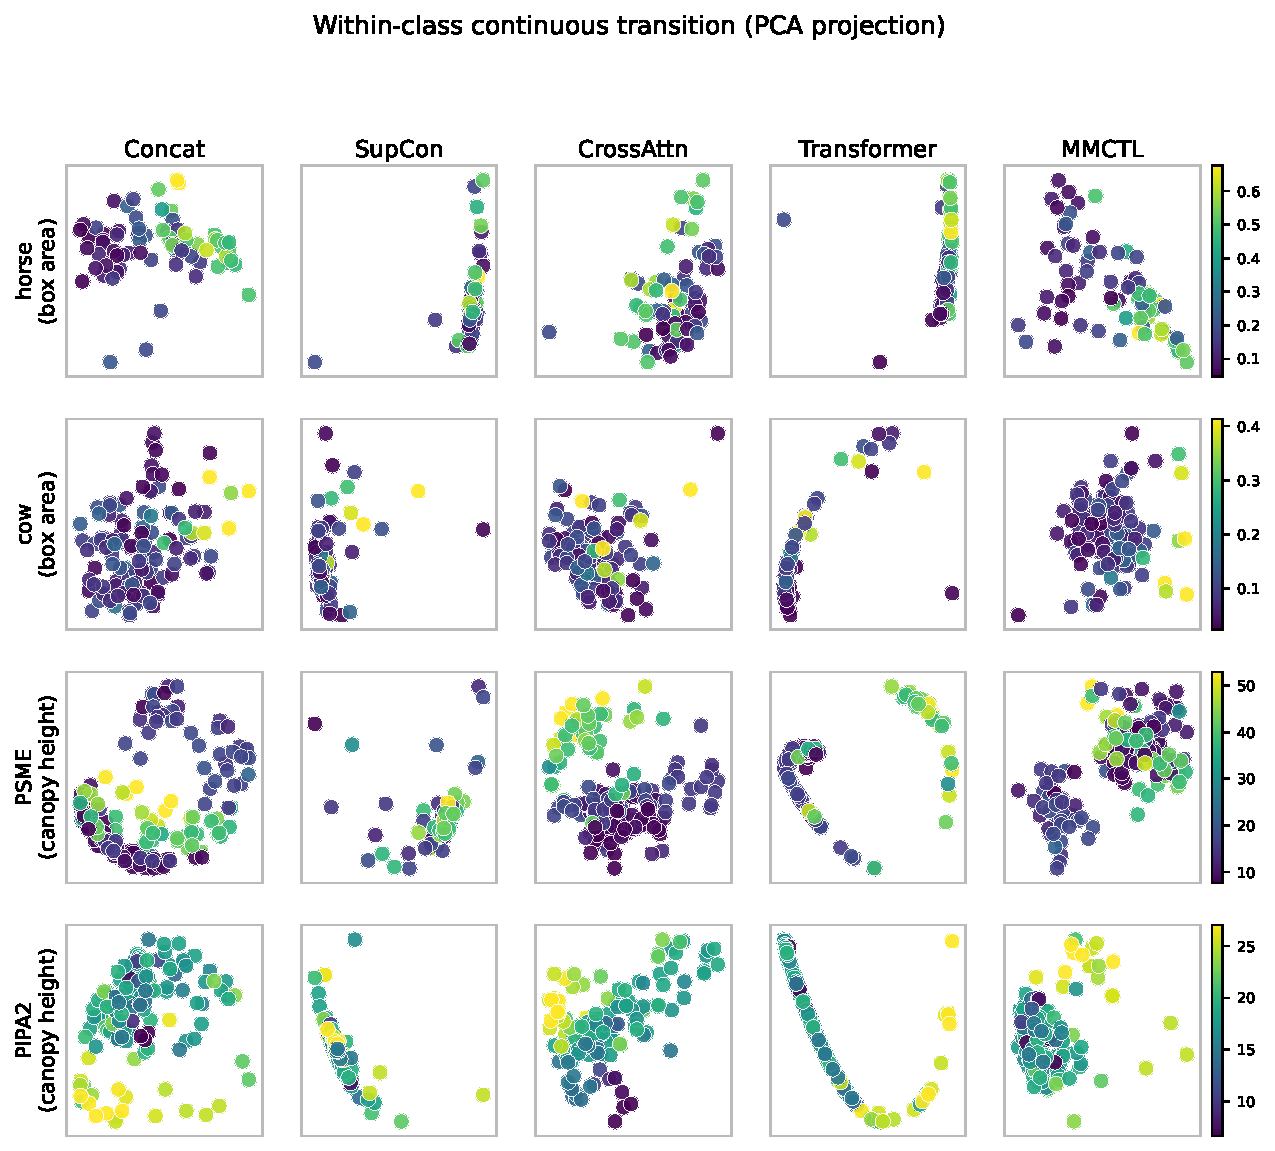
\includegraphics[width=\textwidth]{figures/embedding_zoom_perclass.pdf}
    \caption{\new{Per-class continuous transition. Each row zooms into one class cluster (AWIR horse, cow; NEON PSME, PIPA2) and shows only that class's points under each fusion method (PCA projection), colored by the continuous label indicated at left (box area or canopy height; per-row colorbar). A smooth color gradient across a panel indicates that the continuous attribute varies smoothly within the class embedding. Within-class correlations are reported in Table~\ref{tab:perclass_smooth}.}}
    \label{fig:emb_zoom}
\end{figure*}

\begin{table}[t]
\centering
\caption{\new{Within-class continuous-transition score: Spearman $\rho$ between pairwise cosine embedding distances and pairwise differences of the continuous label, per class and dataset-wide (\emph{All}); higher is smoother. Best method per row in bold; $\star$ marks the classes featured in Fig.~\ref{fig:emb_zoom}.}}
\label{tab:perclass_smooth}
{\color{red}
\footnotesize
\setlength{\tabcolsep}{5pt}
\begin{tabular}{l c c c c c c}
\toprule
\textbf{Class} & \textbf{n} & \textbf{Concat} & \textbf{SupCon} & \textbf{CrsAttn} & \textbf{Trans} & \textbf{MMCTL} \\
\midrule
\multicolumn{7}{l}{\emph{AWIR --- box area}} \\
\emph{All} & 240 & 0.233 & 0.209 & 0.188 & 0.238 & \textbf{0.272} \\
cow$^\star$ & 116 & \textbf{0.289} & 0.201 & 0.190 & 0.254 & 0.212 \\
deer & 51 & 0.040 & \textbf{0.124} & 0.115 & 0.048 & 0.105 \\
horse$^\star$ & 73 & \textbf{0.584} & 0.078 & 0.437 & 0.575 & 0.361 \\
\midrule
\multicolumn{7}{l}{\emph{NEON --- box area}} \\
\emph{All} & 592 & 0.037 & 0.011 & 0.236 & \textbf{0.533} & 0.202 \\
ABLA & 30 & 0.092 & -0.015 & 0.196 & 0.247 & \textbf{0.432} \\
ACRU & 29 & -0.006 & 0.033 & \textbf{0.054} & 0.053 & 0.050 \\
BENE4 & 36 & 0.169 & -0.089 & \textbf{0.299} & 0.235 & 0.173 \\
PIEN & 36 & \textbf{0.236} & -0.010 & 0.188 & 0.145 & 0.057 \\
PIMA & 42 & 0.252 & 0.281 & 0.363 & \textbf{0.384} & 0.291 \\
PIPA2 & 138 & 0.145 & 0.054 & 0.266 & \textbf{0.665} & 0.344 \\
PIPO & 24 & -0.094 & -0.146 & 0.058 & \textbf{0.269} & -0.005 \\
POTR5 & 44 & 0.134 & 0.066 & \textbf{0.276} & 0.273 & 0.128 \\
PSME & 183 & 0.115 & 0.185 & 0.393 & \textbf{0.538} & 0.415 \\
TSCA & 30 & 0.170 & -0.124 & 0.192 & \textbf{0.562} & 0.280 \\
\midrule
\multicolumn{7}{l}{\emph{NEON --- canopy height}} \\
\emph{All} & 592 & 0.121 & 0.066 & 0.252 & \textbf{0.478} & 0.274 \\
ABLA & 30 & \textbf{0.380} & -0.089 & 0.346 & 0.117 & 0.298 \\
ACRU & 29 & -0.009 & -0.044 & \textbf{0.230} & -0.037 & 0.118 \\
BENE4 & 36 & 0.155 & -0.108 & \textbf{0.181} & 0.107 & 0.142 \\
PIEN & 36 & \textbf{0.387} & -0.050 & 0.224 & 0.041 & 0.371 \\
PIMA & 42 & \textbf{0.602} & 0.129 & 0.424 & 0.439 & 0.593 \\
PIPA2$^\star$ & 138 & 0.310 & 0.185 & 0.171 & 0.298 & \textbf{0.504} \\
PIPO & 24 & 0.102 & 0.272 & \textbf{0.355} & 0.150 & 0.017 \\
POTR5 & 44 & 0.633 & 0.351 & \textbf{0.826} & 0.555 & 0.667 \\
PSME$^\star$ & 183 & 0.300 & 0.266 & 0.563 & \textbf{0.662} & 0.593 \\
TSCA & 30 & 0.023 & -0.011 & -0.026 & \textbf{0.187} & 0.127 \\
\bottomrule
\end{tabular}
}
\end{table}

\begin{table}[t]
\centering
\caption{\new{
Downstream task performance using unimodal and fused embeddings. Higher values indicate better performance. Annotation types include C for class labels, B for box, P for position, and H for height annotations.
}}
\label{tab:downstream_performance_tasks}
{\color{red}
\setlength{\tabcolsep}{4pt}
\resizebox{\columnwidth}{!}{%
\begin{tabular}{l c c c c}
\toprule
\textbf{Dataset} & \textbf{Method}
& \textbf{C (\%)} $\uparrow$
& \textbf{B $R^2$} $\uparrow$
& \textbf{P $R^2$} $\uparrow$ \\
\midrule
\multirow{7}{*}{AWIR}
& RGB        
& $79.48 \err{1.50}$ 
& $0.41 \err{0.05}$ 
& $0.23 \err{0.08}$ \\
& Thermal    
& $76.98\err{3.14}$ 
& $0.29\err{0.03}$ 
& $0.01 \err{0.04}$ \\
\cmidrule(lr){2-5}
& Concat.    
& $85.21 \err{2.16}$ 
& $0.45\err{0.02}$ 
& $0.27 \err{0.02}$ \\
& SupCon  
& $89.06 \err{1.47}$ 
& $-0.15\err{0.25}$ 
& $-0.37 \err{0.18}$ \\
& CrossAttn    
& $86.67 \err{1.38}$ 
& $0.31\err{0.06}$ 
& $0.06 \err{0.08}$ \\
& Transformer    
& $86.25 \err{1.50}$ 
& $0.04\err{0.12}$ 
& $-0.16 \err{0.13}$ \\
\cmidrule(lr){2-5}
& MMCTL      
& $\mathbf{91.46}\err{1.49}$ 
& $\mathbf{0.62}\err{0.02}$ 
& $\mathbf{0.50}\err{0.05}$ \\
\midrule
\multicolumn{2}{l}{}
& \textbf{C (\%)} $\uparrow$
& \textbf{B $R^2$} $\uparrow$
& \textbf{H $R^2$} $\uparrow$ \\
\midrule
\multirow{8}{*}{NEON}
& RGB        
& $76.22\err{2.33}$ 
& $0.07 \err{0.09}$ 
& $0.32 \err{0.03}$ \\
& HSI        
& $76.22 \err{1.38}$ 
& $0.13 \err{0.06}$ 
& $0.40\err{0.03}$ \\
& LiDAR      
& $48.38 \err{2.09}$ 
& $0.15 \err{0.08}$ 
& $0.67 \err{0.02}$ \\
\cmidrule(lr){2-5}
& Concat.    
& $80.81 \err{1.96}$ 
& $\mathbf{0.36} \err{0.08}$ 
& $\mathbf{0.71} \err{0.01}$ \\
& SupCon  
& $\mathbf{81.42} \err{1.97}$ 
& $0.07 \err{0.14}$ 
& $0.47 \err{0.06}$ \\
& CrossAttn    
& $68.85 \err{2.17}$ 
& $0.27\err{0.10}$ 
& $0.60 \err{0.03}$ \\
& Transformer    
& $43.11 \err{4.50}$ 
& $0.24\err{0.13}$ 
& $0.29 \err{0.06}$ \\
\cmidrule(lr){2-5}  
& MMCTL      
& $80.34 \err{1.03}$ 
& $0.33 \err{0.05}$ 
& $0.63 \err{0.03}$ \\
\bottomrule
\end{tabular}}
}
\end{table}


\subsection{\new{Annotation Weighting and Frozen vs.\ End-to-End Encoders}}
\label{subsec:weight-e2e}

\new{\noindent\textbf{Class-weight sensitivity (NEON).}
The joint annotation vector exposes one free knob per task, the weight $w_t$ (Eq.~\eqref{eq:ann-weight}). We sweep the class weight $w_{\text{class}}\in\{0.5,0.8,1.0,1.5\}$ on NEON with the continuous-task weights fixed at $1.0$, using the released full-set MMCTL embeddings under the frozen task-head protocol. As shown in Fig.~\ref{fig:neon_ablation} and Table~\ref{tab:neon_weight_ablation}, increasing $w_{\text{class}}$ sharpens species separation in the embedding space and improves classification accuracy, with a mild trade-off against continuous-attribute regression. This confirms that the weight behaves as intended---trading semantic compactness against geometric spread---and motivates the balanced default used in the main tables.}

\begin{figure*}[!htb]
    \centering
    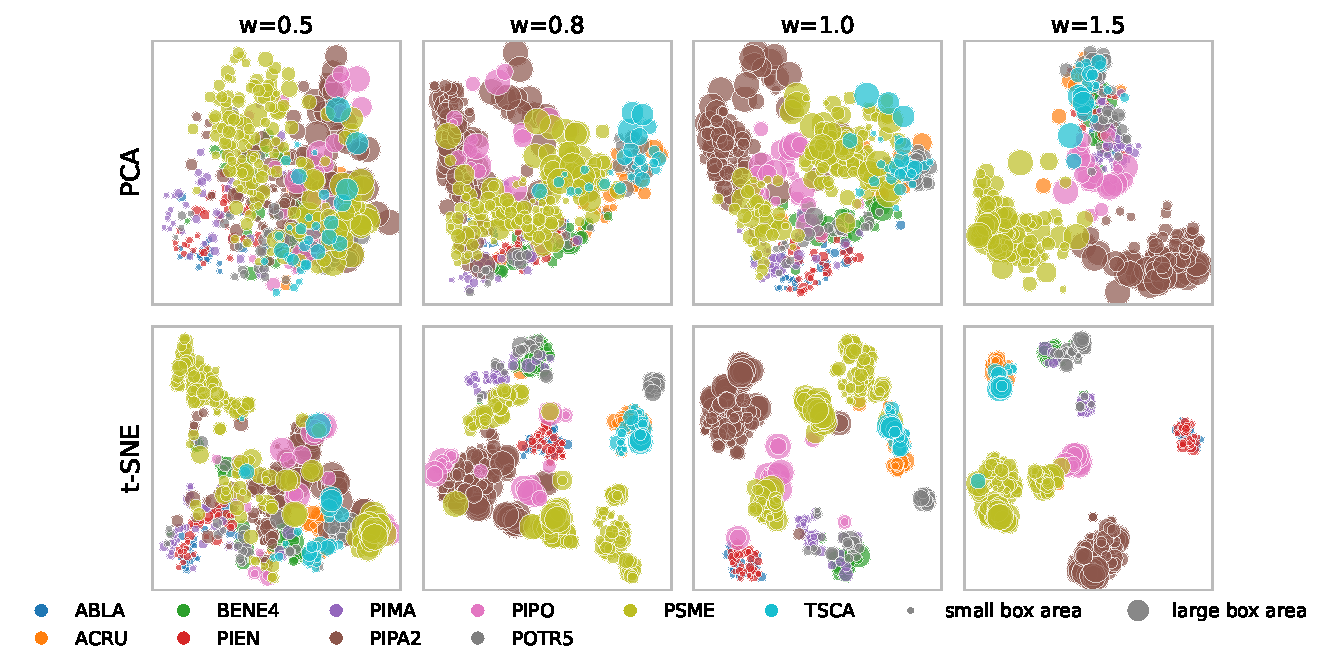
\includegraphics[width=\textwidth]{figures/neon_ablation_classweight_boxsize.pdf}
    \caption{\new{NEON class-weight ablation. MMCTL embeddings trained with class weight $w_{\text{class}}\in\{0.5,0.8,1.0,1.5\}$ (box/height weights fixed at $1.0$), projected with PCA (top) and t-SNE (bottom), colored by species and sized by bounding-box area. Larger class weights yield more compact, better-separated species clusters. (A height-sized version is provided in the supplementary figures.)}}
    \label{fig:neon_ablation}
\end{figure*}

\begin{table}[t]
\centering
\caption{\new{NEON class-weight ablation (R1.4). MMCTL trained with class-label weight $w_{\text{class}}$ swept while box/height weights are fixed at $1.0$; frozen task-head protocol, mean$\pm$std over $5$ folds. Increasing $w_{\text{class}}$ steadily improves classification while box/height regression stays stable, trading semantic compactness against continuous spread. Best per column in bold.}}
\label{tab:neon_weight_ablation}
{\color{red}
\begin{tabular}{c c c c}
\toprule
$w_{\text{class}}$ & \textbf{Acc (\%)} $\uparrow$ & \textbf{Box $R^2$} $\uparrow$ & \textbf{Height $R^2$} $\uparrow$ \\
\midrule
$0.5$ & $74.86\err{1.24}$ & $0.167\err{0.043}$ & $\mathbf{0.663}\err{0.021}$ \\
$0.8$ & $79.32\err{1.78}$ & $0.203\err{0.062}$ & $0.602\err{0.022}$ \\
$1.0$ & $80.14\err{2.18}$ & $\mathbf{0.283}\err{0.044}$ & $0.653\err{0.025}$ \\
$1.5$ & $\mathbf{84.59}\err{1.43}$ & $0.252\err{0.076}$ & $0.619\err{0.028}$ \\
\bottomrule
\end{tabular}
}
\end{table}

\new{\noindent\textbf{Frozen vs.\ end-to-end encoders (NEON).}
The main protocol freezes modality encoders and trains task heads on fixed embeddings. To test whether this frozen choice is justified relative to fine-tuning, we run a controlled comparison on NEON: starting from the same MMCTL-pretrained encoders, we either keep them frozen (main protocol) or unfreeze them and fine-tune end-to-end jointly with the heads, holding the head architecture, data splits, standardized targets, and training budget fixed so the only difference is encoder trainability. Averaged over the five folds, freezing matches or exceeds end-to-end fine-tuning: classification accuracy is $81.99\pm1.02\%$ (frozen) vs.\ $80.66\pm1.35\%$ (end-to-end), while end-to-end yields only marginal gains on the continuous heads (box $R^2$ $0.316\pm0.040\rightarrow0.344\pm0.068$; height $R^2$ $0.514\pm0.091\rightarrow0.572\pm0.034$). Fine-tuning the encoders therefore does not improve, and slightly degrades, classification, confirming that the frozen protocol is a sound and substantially cheaper default rather than a limitation of the method.}

\subsection{\red{Missing Modality and Compute}}
\label{subsec:additional-analyses}

\new{\noindent\textbf{Missing modality.} As a frozen-embedding probe on released AWIR test embeddings, we zero one $1024$-d half of the $2048$-d MMCTL joint vector (RGB$|$thermal), L2-normalize, and retrain linear probes. Full joint proxy accuracy is $93.44\pm1.37\%$. Dropping thermal yields $84.69\pm2.04\%$ ($-8.75$~pts); dropping RGB yields $86.15\pm1.99\%$ ($-7.29$~pts). Both remain above unimodal RGB/thermal probe accuracies ($\approx$78--80\%), indicating complementary but non-redundant modality use under this probe protocol.}

\new{\noindent\textbf{Triplet compute.} With batch size $32$, modality concatenation yields $64$ embeddings and an upper bound of $249{,}984$ ordered triplets per batch ($\approx 2.0$M per epoch at eight steps) before the annotation-order mask; actual positives are data-dependent. A microbenchmark on Apple M4 CPU measures $\approx 1.7$\,s per training step at batch size $8$; the full AWIR training schedule was not re-timed on this machine.}


\section{Conclusion}
This work frames multi-modal representation learning as aligning embeddings across sensing modalities using annotation-defined similarity rather than task-loss geometry alone. MMCTL builds a shared latent space by coupling modality-specific embeddings through a weighted joint annotation vector, a margin-free continuous triplet, and pairwise distance alignment, yielding more coherent cross-modal geometry than unimodal or task-driven fusion under the same label sources. AWIR analyses further show statistically significant structure gains and graceful degradation under missing-modality probes. Future work includes adaptive annotation weights that adjust task influence during training.


{
    \small
    \bibliographystyle{ieeenat_fullname}
    \bibliography{paper}
}

\end{document}
